% PGF/TikZ manual, pgfmanual-en-library-petri.tex:65-72.
% Copyright 2019 Till Tantau. LPPL and/or GNU Free Documentation License.
\documentclass[border=2pt]{standalone}
\usepackage{tikz}
\usetikzlibrary{petri,positioning}
\begin{document}
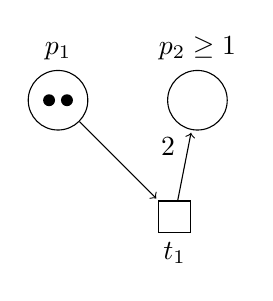
\begin{tikzpicture}
  \node[place,tokens=2,label=above:$p_1$]        (p1) {};
  \node[place,label=above:$p_2\ge1$,right=of p1] (p2) {};

  \node[transition,below right=of p1,label=below:$t_1$] {}
    edge[pre]                 (p1)
    edge[post] node[auto] {2} (p2);
\end{tikzpicture}
\end{document}
